\documentclass[12pt, a4paper]{report}
\usepackage[utf8]{inputenc}
\usepackage[english, russian]{babel}

\usepackage{graphicx}
\usepackage{listings}
\usepackage{color}

\usepackage{amsmath}
\usepackage{pgfplots}
\usepackage{url}
\usepackage{flowchart}
\usepackage{tikz}
\DeclareGraphicsExtensions{.pdf,.png,.jpg,.svg}
\usetikzlibrary{shapes, arrows}

\usepackage{pgfplotstable}

\renewcommand\contentsname{Содержание}

\usepackage{geometry}
\geometry{left=3cm}
\geometry{right=1cm}
\geometry{top=2cm}
\geometry{bottom=2cm}

\lstset{ %
language=Python,                 % выбор языка для подсветки (здесь это С)
basicstyle=\small\sffamily, % размер и начертание шрифта для подсветки кода
numbers=left,               % где поставить нумерацию строк (слева\справа)
numberstyle=\tiny,           % размер шрифта для номеров строк
stepnumber=1,                   % размер шага между двумя номерами строк
numbersep=-5pt,                % как далеко отстоят номера строк от         подсвечиваемого кода
backgroundcolor=\color{white}, % цвет фона подсветки - используем         \usepackage{color}
showspaces=false,            % показывать или нет пробелы специальными     отступами
showstringspaces=false,      % показывать или нет пробелы в строках
showtabs=false,             % показывать или нет табуляцию в строках
frame=single,              % рисовать рамку вокруг кода
tabsize=2,                 % размер табуляции по умолчанию равен 2 пробелам
captionpos=t,              % позиция заголовка вверху [t] или внизу [b] 
breaklines=true,           % автоматически переносить строки (да\нет)
breakatwhitespace=false, % переносить строки только если есть пробел
escapeinside={\%*}{*)},   % если нужно добавить комментарии в коде
keywordstyle=\color{blue}\ttfamily,
stringstyle=\color{red}\ttfamily,
commentstyle=\color{green}\ttfamily,
morecomment=[l][\color{magenta}]{\#},
columns=fullflexible }

\usepackage{titlesec}
\titleformat{\chapter}[hang]{\LARGE\bfseries}{\thechapter{.} }{0pt}{\LARGE\bfseries}
\titleformat*{\section}{\Large\bfseries}
\titleformat*{\subsection}{\large\bfseries}

\begin{document}

    \begin{titlepage}

        \begin{center}
            \Large
            {\sl Государственное образовательное учреждение высшего профессионального образования\\
            {\bf«Московский государственный технический университет имени Н.Э. Баумана»\\
				(МГТУ им. Н.Э. Баумана)}}
            \vspace{3cm}

			{\scshape\LARGE Рубежный контроль №2 \par}
			\vspace{0.5cm}	
			{\scshape\LARGE по курсу «Анализ алгоритмов» \par}
			\vspace{1.5cm}
			{\huge\bfseries Конечные автоматы и регулярные выражения \par}
			\vspace{2cm}
			\Large Выполнил: Харламов П.С., гр. ИУ7-55Б\\
			\vspace{0.5cm}
			{\Large Преподаватели: Волкова Л.Л., Строганов Ю.В.}
		
			\vfill
			\Large \textit {2020 г.}
            
        \end{center}

    \end{titlepage}
	
	\tableofcontents

	\chapter*{Введение}
	\addcontentsline{toc}{chapter}{Введение}
	
	Задача лабораторной работы состоит в том, что нужно при помощи конечного автомата и регулярного выражения написать программу поиска всех групп вуза: для специалитета, бакалавров, магистров в тексте.
	

    \chapter{Аналитический раздел}
   	\vspace{-0.5cm}В данном разделе будут описаны конечные автоматы и регулярные выражения.
	\section{Конечные автоматы}
	Конечные автоматы - это до предела упрощенная модель компьютера имеющая конечное число состояний, которая жертвует всеми особенностями компьютеров такие как ОЗУ, постоянная память, устройства ввода-вывода и процессорными ядрами в обмен на простоту понимания, удобство рас­суждения и легкость программной или аппаратной реализации\cite{fsm}.
	
	С помощью КА можно реализовать такие вещи как, регулярные выражения, лексический анализатор, ИИ в играх и тд.
	
	Для реализации поставленной задачи был спроектирован конечный автомат, представленный на рисунке \ref{pic:fsm}
	
	\begin{figure}[ht!]
		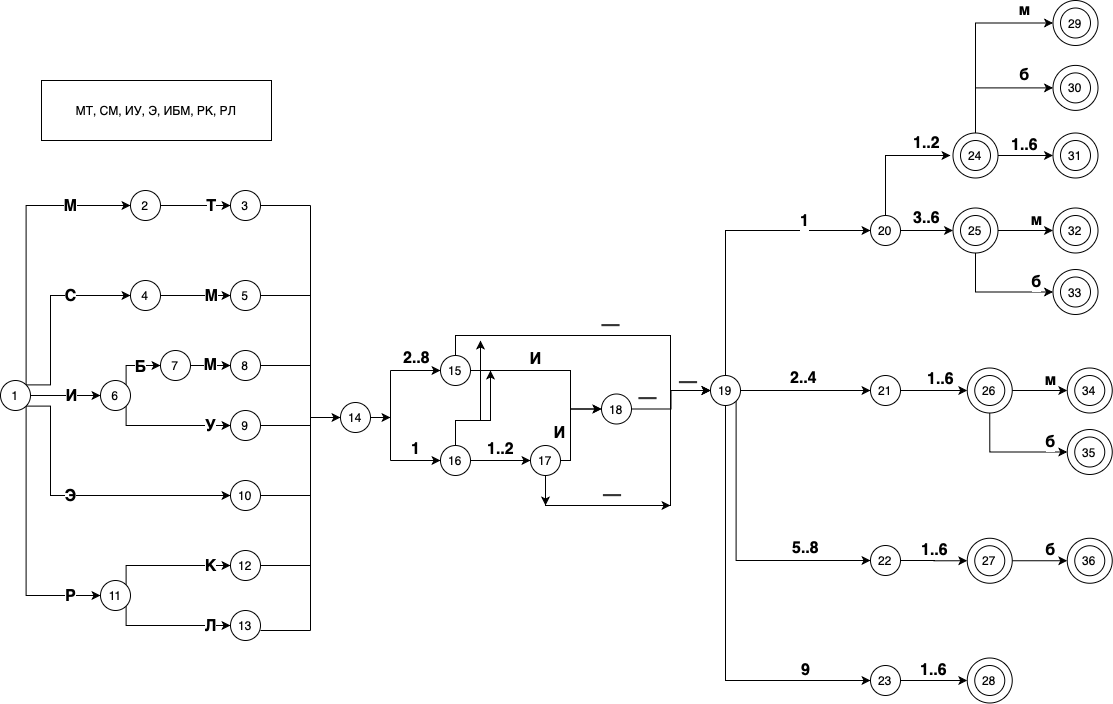
\includegraphics[scale=0.4]{fsm.png}
		\caption{Конечный автомат для поиска группы вуза}
		\label{pic:fsm}
	\end{figure}

	\section{Регулярные выражения}
	
	Регулярные выражения — язык поиска подстроки или подстрок в тексте. Для поиска используется паттерн (шаблон, маска), состоящий из символов и метасимволов (символы, которые обозначают не сами себя, а набор символов).
	
	Это довольно мощный инструмент, который может пригодиться во многих случая — поиск, проверка на корректность строки и т.д. Спектр его возможностей трудно уместить в одну статью\cite{regular}.
	
	Для реализации поставленной задачи был спроектировано регулярное выражение по образу конечный автомата, представленного на рисунке \ref{pic:fsm}
	
	$$(\text{МТ+И(У + БМ)+Р(Л + К + КТ)+}$$
	$$\text{+ФН+С(М + ГН)+Э+БМТ+Л+АК})(1 + ... + 12)\text{(И + ' ')} -$$
	$$-(1 + ... + 12)(\text{Б + М + б + м + ' '})$$
	
	\section{Вывод}
	В данном разделе были описаны конечные автоматы и регулярные выражения.

	
	\chapter{Технологический раздел}
	\vspace{-0.5cm}В данном разделе будут предъявлены требования к программному обеспечению, средства реализации и листинги кода.
	
	\section{Требования к программному обеспечению}
	Программное обеспечение должно реализовавать поиск подстроки в строке с помощью конечного автомата и регулярного выражения. Причем, для конечного автомата не должно исполизоваться никаких библиотек, а реализация регулярного выражения может быть осуществлена с использованием библиотек.
	\section{Средства реализации}
	Для выполнения поставленной задачи был использован язык программирования Python. Среда для разработки IDLE. Для измерения времени была взята функция time.time() из библиотеки time.
	
	\vspace{0.2cm}Данный язык обусловлен тем, что функции необходимые для реализации регулярного выражения находятся в встроенной библиотеке re.
	
	
	\section{Листинг кода}
	В данном подразделе представлены листинги кода реализации конечного автомата и регулярного выражения, которые были представлены в аналитическом разделе.

	\begin{lstlisting}[label=code:fsm,caption=Реализация конечного автомата]
	import time
	
	def GetFSM(stroke):
	
	state = 1
	groupName = ''
	
	for value in stroke:
	# print(state)
	# print("value = " + value)
	if state == 1:
	if value  ==  'M':
	state = 2
	elif value == 'C':
	state = 4
	elif value == 'N':
	state = 6
	elif value == 'E':
	state = 14
	elif value == 'P':
	state = 11
	else:
	break
	groupName += value
	
	elif state == 2:
	if value == 'T':
	state = 14
	else:
	break
	groupName += value
	
	elif state == 4:
	if value == 'M':
	state = 14
	else:
	break
	groupName += value
	
	elif state == 6:
	if value == 'B':
	state = 7
	elif value == 'Y':
	state = 14
	else:
	break
	groupName += value
	
	elif state == 11:
	if value == 'K':
	state = 14
	elif value == 'L':
	state = 14
	else:
	break
	groupName += value
	
	elif state == 7:
	if value == 'M':
	state = 14
	else:
	break
	groupName += value
	
	elif state == 14:
	if value.isdigit() and int(value) in [2,3,4,5,6,7,8] :
	state = 15
	elif value.isdigit() and int(value) == 1:
	state = 16
	else:
	break
	groupName += value
	
	elif state == 15:
	if value == '-':
	state = 19
	elif value == 'N':
	state = 18
	else:
	break
	groupName += value
	
	elif state == 16:
	if value.isdigit() and int(value) in [1,2]:
	state = 17
	elif value == 'N':
	state = 18
	elif value == '-':
	state = 19
	else:
	break
	groupName += value
	
	elif state == 17:
	if value == 'N':
	state = 18
	elif value == '-':
	state = 19
	else:
	break
	groupName += value
	
	elif state == 18:
	if value == '-':
	state = 19
	else:
	break
	length += 1
	
	elif state == 19:
	if value.isdigit() and int(value) in [1]:
	state = 20
	elif value.isdigit() and int(value) in [2,3,4]:
	state = 21
	elif value.isdigit() and int(value) in [5,6,7,8]:
	state = 22
	elif value.isdigit() and int(value) in [9]:
	state = 23
	else:
	break
	groupName += value
	
	elif state == 20:
	if value.isdigit() and int(value) in [1,2]:
	state = 24
	elif value.isdigit() and int(value) in [3,4,5,6]:
	state = 25
	else:
	break
	groupName += value
	
	elif state == 21:
	if value.isdigit() and int(value) in [1,2,3,4,5,6]:
	state = 26
	else:
	break
	groupName += value
	
	elif state == 22:
	if value.isdigit() and int(value) in [1,2,3,4,5,6]:
	state = 27
	else:
	break
	groupName += value
	
	elif state == 23:
	if value.isdigit() and int(value) in [1,2,3,4,5,6]:
	state = 28
	else:
	break
	groupName += value
	
	elif state == 24:
	if value == "M":
	state = 29
	elif value == "B":
	state = 30
	elif value.isdigit() and int(value) in [1,2,3,4,5,6]:
	state = 31
	else:
	break
	groupName += value
	
	elif state == 25:
	if value == "M":
	state = 32
	elif value == "B":
	state = 33
	else:
	break
	groupName += value
	
	elif state == 26:
	if value == "M":
	state = 34
	elif value == "B":
	state = 35
	else:
	break
	groupName += value
	
	elif state == 27:
	if value == "B":
	state = 36
	else:
	break
	groupName += value
	
	# print("State = " + str(state))
	# print("Group = " + str(groupName))
	
	if state >= 24 and state <= 36:
	return groupName
	else: return ''
	
	def FindGroups(text):
	
	groups = []
	text += "*******"
	
	i = 0
	
	while(1):
	
	if len(text) <= i + 10:
	break
	
	tmpStroke = text[i: i + 10]
	tmpStroke = tmpStroke.upper()
	
	group = GetFSM(tmpStroke)
	if group != '':
	groups.append(group)
	
	i += 1
	
	return groups
	
	if __name__ == '__main__':
	f = open('/kek/text.txt', 'r')
	
	text = f.read()
	
	f.close()
	
	start_time = time.time()
	
	findedGroups = FindGroups(text)
	
	totalTime = time.time() - start_time
	totalTime = round(totalTime * 1000, 4)
	print("--- %s seconds ---" % totalTime)
	
	# for group in findedGroups:
	#     print(group)
	\end{lstlisting}
	
	\begin{lstlisting}[label=code:regular,caption=Реализация регулярного выражения]
	import re
	import time
	
	def FindGroups(text, doPrint):
	
	text += "*******"
	
	i = 0
	
	while(1):
	
	if len(text) <= i + 10:
	break
	
	tmpStroke = text[i: i + 10]
	tmpStroke = tmpStroke.upper()
	
	match = re.match(r'(MT|IU|RL|FN|CM|E|RK|BMT|IBM|L|SGN|RKT|AK)(10|11|12|[1-9])-((10|11|12|[1-9]))[1-6][bmBM]?',
	tmpStroke)
	
	if doPrint == 1 and match != None:
	print(match[0])
	
	i += 1
	
	
	if __name__ == '__main__':
	
	f = open('/kek/text.txt', 'r')
	
	text = f.read()
	
	f.close()
	
	start_time = time.time()
	
	FindGroups(text, 0)
	
	totalTime = time.time() - start_time
	totalTime = round(totalTime * 1000, 4)
	print("--- %s seconds ---" % totalTime)
	
	\end{lstlisting}

	\newpage

	\section{Вывод}
	В данном разделе были предъявлены требования к программному обеспечению, средства реализации и листинги кода.


	\newpage

	\chapter*{Заключение}
	\addcontentsline{toc}{chapter}{Заключение}
	Были изучены основные принципы работы регулярных выражений и конечных автоматов для поиска подстроки в тексте, а также разработана программа, решающая задау поиска в тексте групп университета МГТУ им. Баумана.
	
	\newpage
	
	\begin{thebibliography}{}
	\bibitem{fsm}
	Конечные автоматы (finite-state machine) [Электронный ресурс]. - Режим доступа: https://habr.com/ru/post/358304/, свободный. (Дата обращения: 5.2.2020 г.)
	\bibitem{regular}
	Регулярные выражения [Электронный ресурс]. - Режим доступа: https://habr.com/ru/company/badoo/blog/343310/, свободный. (Дата обращения: 5.2.2020 г.)
	\end{thebibliography}
	\addcontentsline{toc}{chapter}{Литература}

\end{document}